\documentclass{beamer}
\begin{document}
\title{KiCAD\\Creating a schematic symbol}
\author{Katharina Fey}
\date{17. March 2018}

\frame{\titlepage}


%%%%%%%%%%%%%%%%%%%%%%%%%%%%%%%%%%%%%%%%%%%%%%%%%%%%%%%%%
\begin{frame}
  \frametitle{Create new symbol}
  \begin{itemize}
    \item Open the schematic symbol editor
    \item Create a new symbol
    \item Alternatively, you can of course load an existing library and add a symbol there
  \end{itemize}
  \begin{figure}[H]
    \centering
    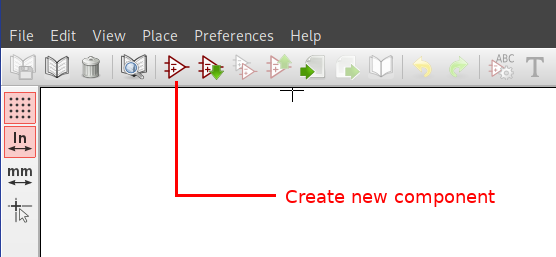
\includegraphics[width=0.95\textwidth]{images/step_01.png}
  \end{figure}
\end{frame}


%%%%%%%%%%%%%%%%%%%%%%%%%%%%%%%%%%%%%%%%%%%%%%%%%%%%%%%%%
\begin{frame}
  \frametitle{Create new symbol}
  \begin{itemize}
    \item Create pins according to the datasheet
    \item Use shapes to make it look nice
  \end{itemize}
  \begin{figure}[H]
    \centering
    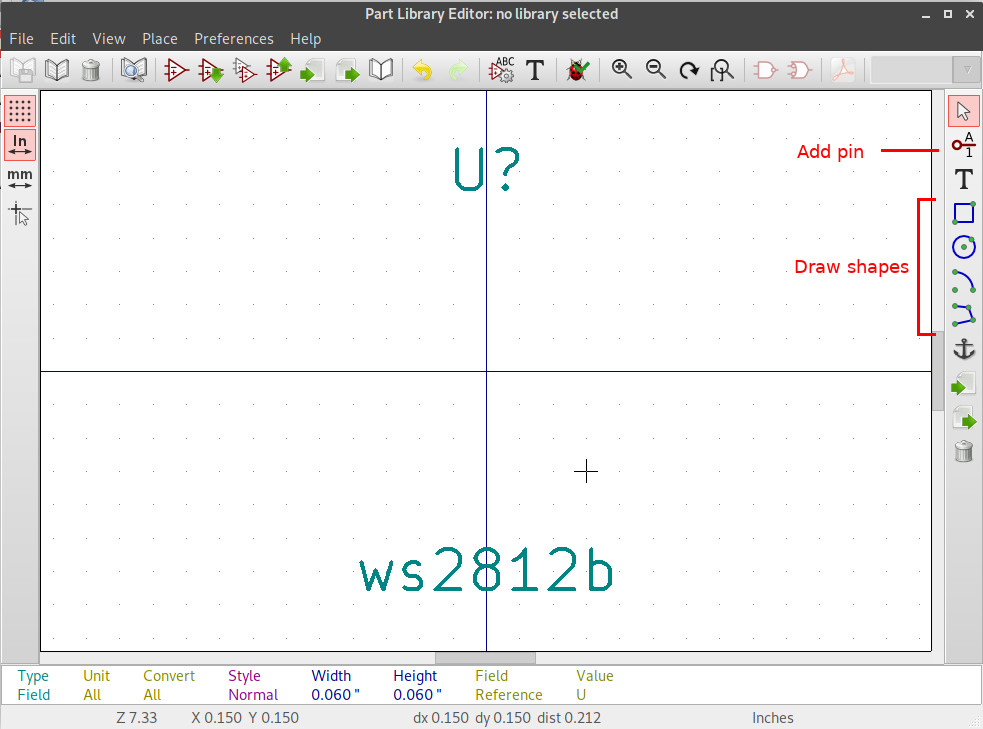
\includegraphics[width=0.75\textwidth]{images/step_02.png}
  \end{figure}
\end{frame}


%%%%%%%%%%%%%%%%%%%%%%%%%%%%%%%%%%%%%%%%%%%%%%%%%%%%%%%%%
\begin{frame}
  \frametitle{Save as new library}
  \begin{itemize}
    \item Because this is the fist symbol, save it as a new library
  \end{itemize}
  \begin{figure}[H]
    \centering
    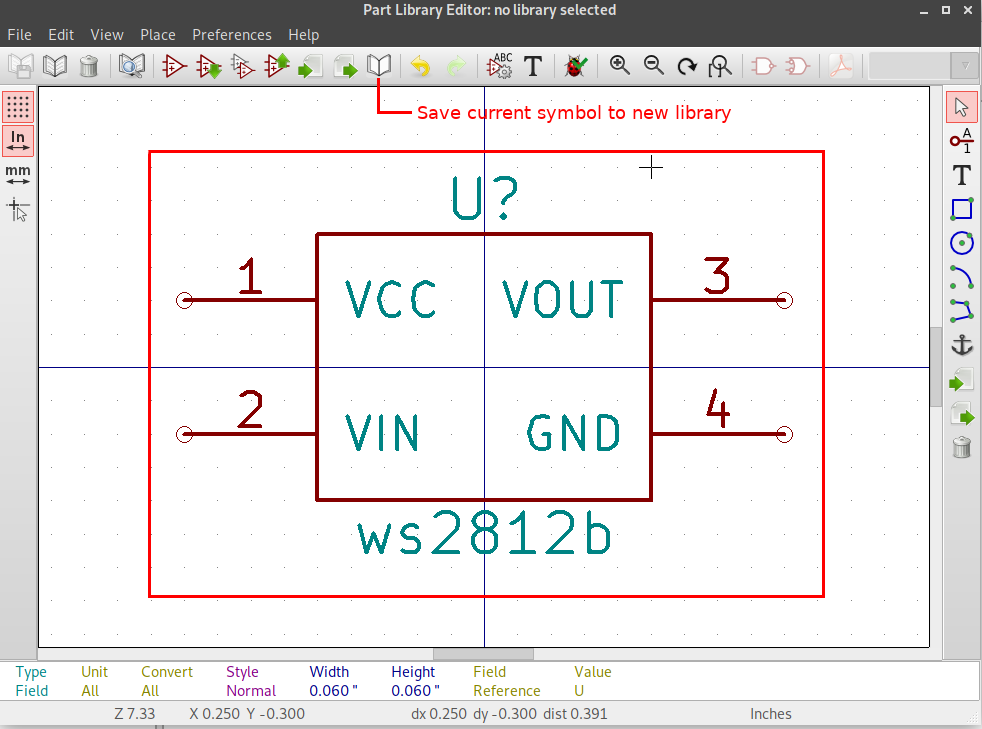
\includegraphics[width=0.75\textwidth]{images/step_03.png}
  \end{figure}
\end{frame}


%%%%%%%%%%%%%%%%%%%%%%%%%%%%%%%%%%%%%%%%%%%%%%%%%%%%%%%%%
\begin{frame}
  \frametitle{Include new library}
  \begin{itemize}
    \item Open library include settings
  \end{itemize}
  \begin{figure}[H]
    \centering
    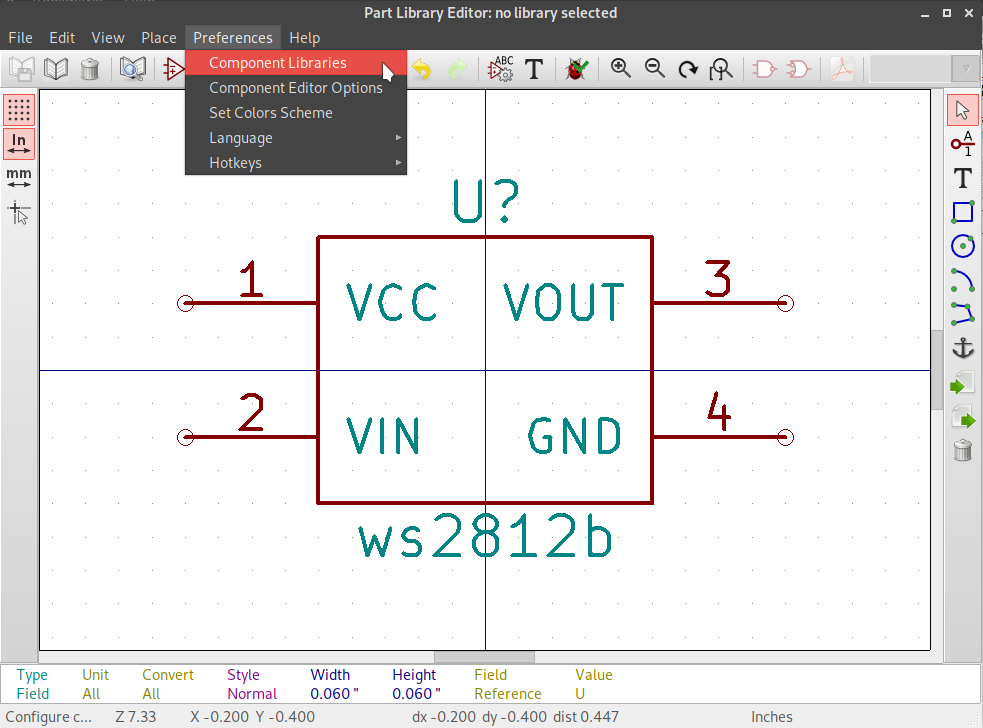
\includegraphics[width=0.75\textwidth]{images/step_04.png}
  \end{figure}
\end{frame}


%%%%%%%%%%%%%%%%%%%%%%%%%%%%%%%%%%%%%%%%%%%%%%%%%%%%%%%%%
\begin{frame}
  \frametitle{Include new library}
  \begin{itemize}
    \item Add the new library to the include path
  \end{itemize}
  \begin{figure}[H]
    \centering
    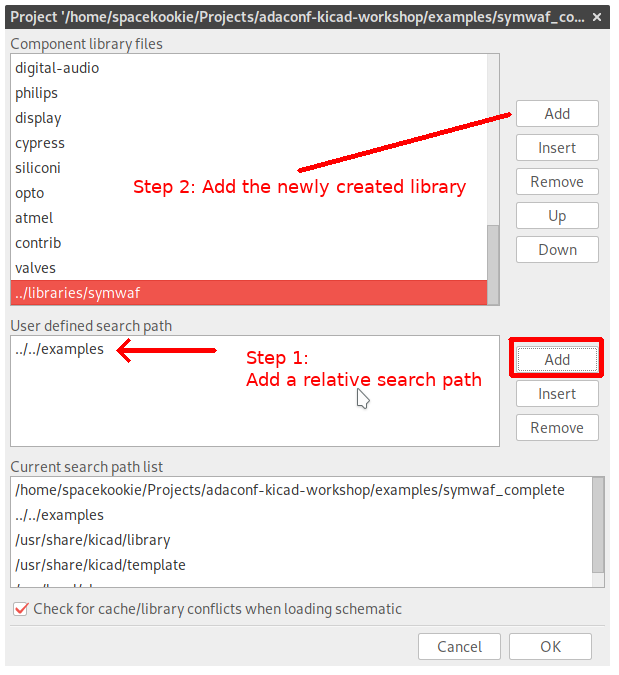
\includegraphics[width=0.55\textwidth]{images/step_05.png}
  \end{figure}
\end{frame}


%%%%%%%%%%%%%%%%%%%%%%%%%%%%%%%%%%%%%%%%%%%%%%%%%%%%%%%%%
\begin{frame}
  \frametitle{Set library as active}
  \begin{itemize}
    \item Load the newly created library to work on it further
  \end{itemize}
  \begin{figure}[H]
    \centering
    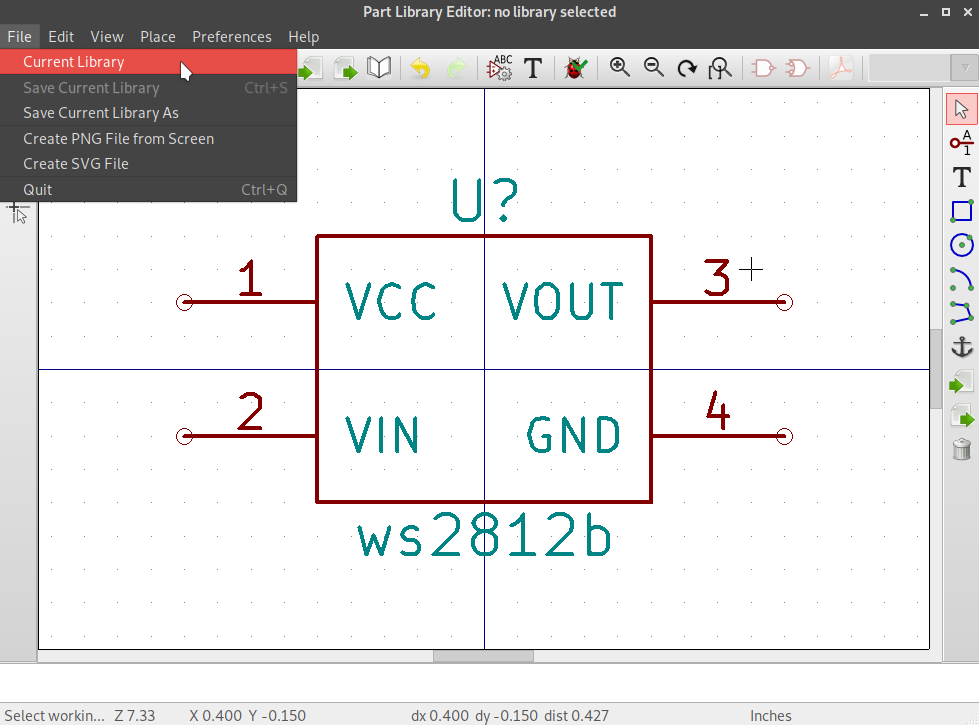
\includegraphics[width=0.55\textwidth]{images/step_06.png}
  \end{figure}
\end{frame}


\end{document}

